\section{Introduction}
\label{sec:intro}

% General motivation.
Machine Learning (ML) and data science have profound impact on many applications in practice. In the past, ML systems primarily focused on efficient model training and prediction. However, there is a trend toward systems support for ML pipelines and the entire data science lifecycle. Systems like KeystoneML \cite{SparksVKFR17}, Amazon SageMaker \cite{LibertyKXRCNDSA20}, Scikit-learn \cite{PedregosaVGMTGBPWDVPCBPD11}, SystemDS \cite{BoehmADGIKLPR20}, and TensorFlow TFX \cite{BaylorBCFFHHIJK17} provide abstractions for data integration, validation, and augmentation, feature extraction and engineering, model selection and hyper-parameter tuning, model training and prediction, as well as model debugging. Integrating these abstractions into ML systems is compelling because state-of-the-art data integration and cleaning largely rely on ML models \cite{DongR18}. However, complex ML pipelines create challenges regarding reproducibility and computational redundancy, which can be addressed with data provenance. 

% Existing work
\textbf{Data Provenance in ML Systems:} Data provenance captures the origin and creation of data for understanding why and how query results were created \cite{GlavicD07,CheneyCT09,Tan07}. Similarly, lineage---in terms of logical data transformations---has also been used for low-overhead fault tolerance in data-parallel frameworks like Apache Spark \cite{ZahariaCDDMMFSS12}. Recently, these concepts were adopted in ML system prototypes such as MISTIQUE \cite{VartakTMZ18}, HELIX \cite{XinMMLSP18}, Alpine Meadow \cite{ShangZBKECBUK19}, and the Collaborative Optimizer (CO) \cite{DerakhshanMARM20} for debugging and reusing intermediates. Existing approaches rely on coarse-grained lineage tracing at the level of ML pipelines and their top-level steps as shown in Figure~\ref{fig:coarsefine}-left. This black-box view of individual pre-processing steps, feature engineering, hyper-parameter tuning, and ML algorithms allows using existing---and rapidly evolving---ML systems. Unfortunately though, this approach fails to detect internal non-determinism and fine-grained redundancy. Exposing the internals of composite primitives at pipeline level is possible but requires a reimplementation of such primitives.

\begin{figure}[!t]
	\centering
	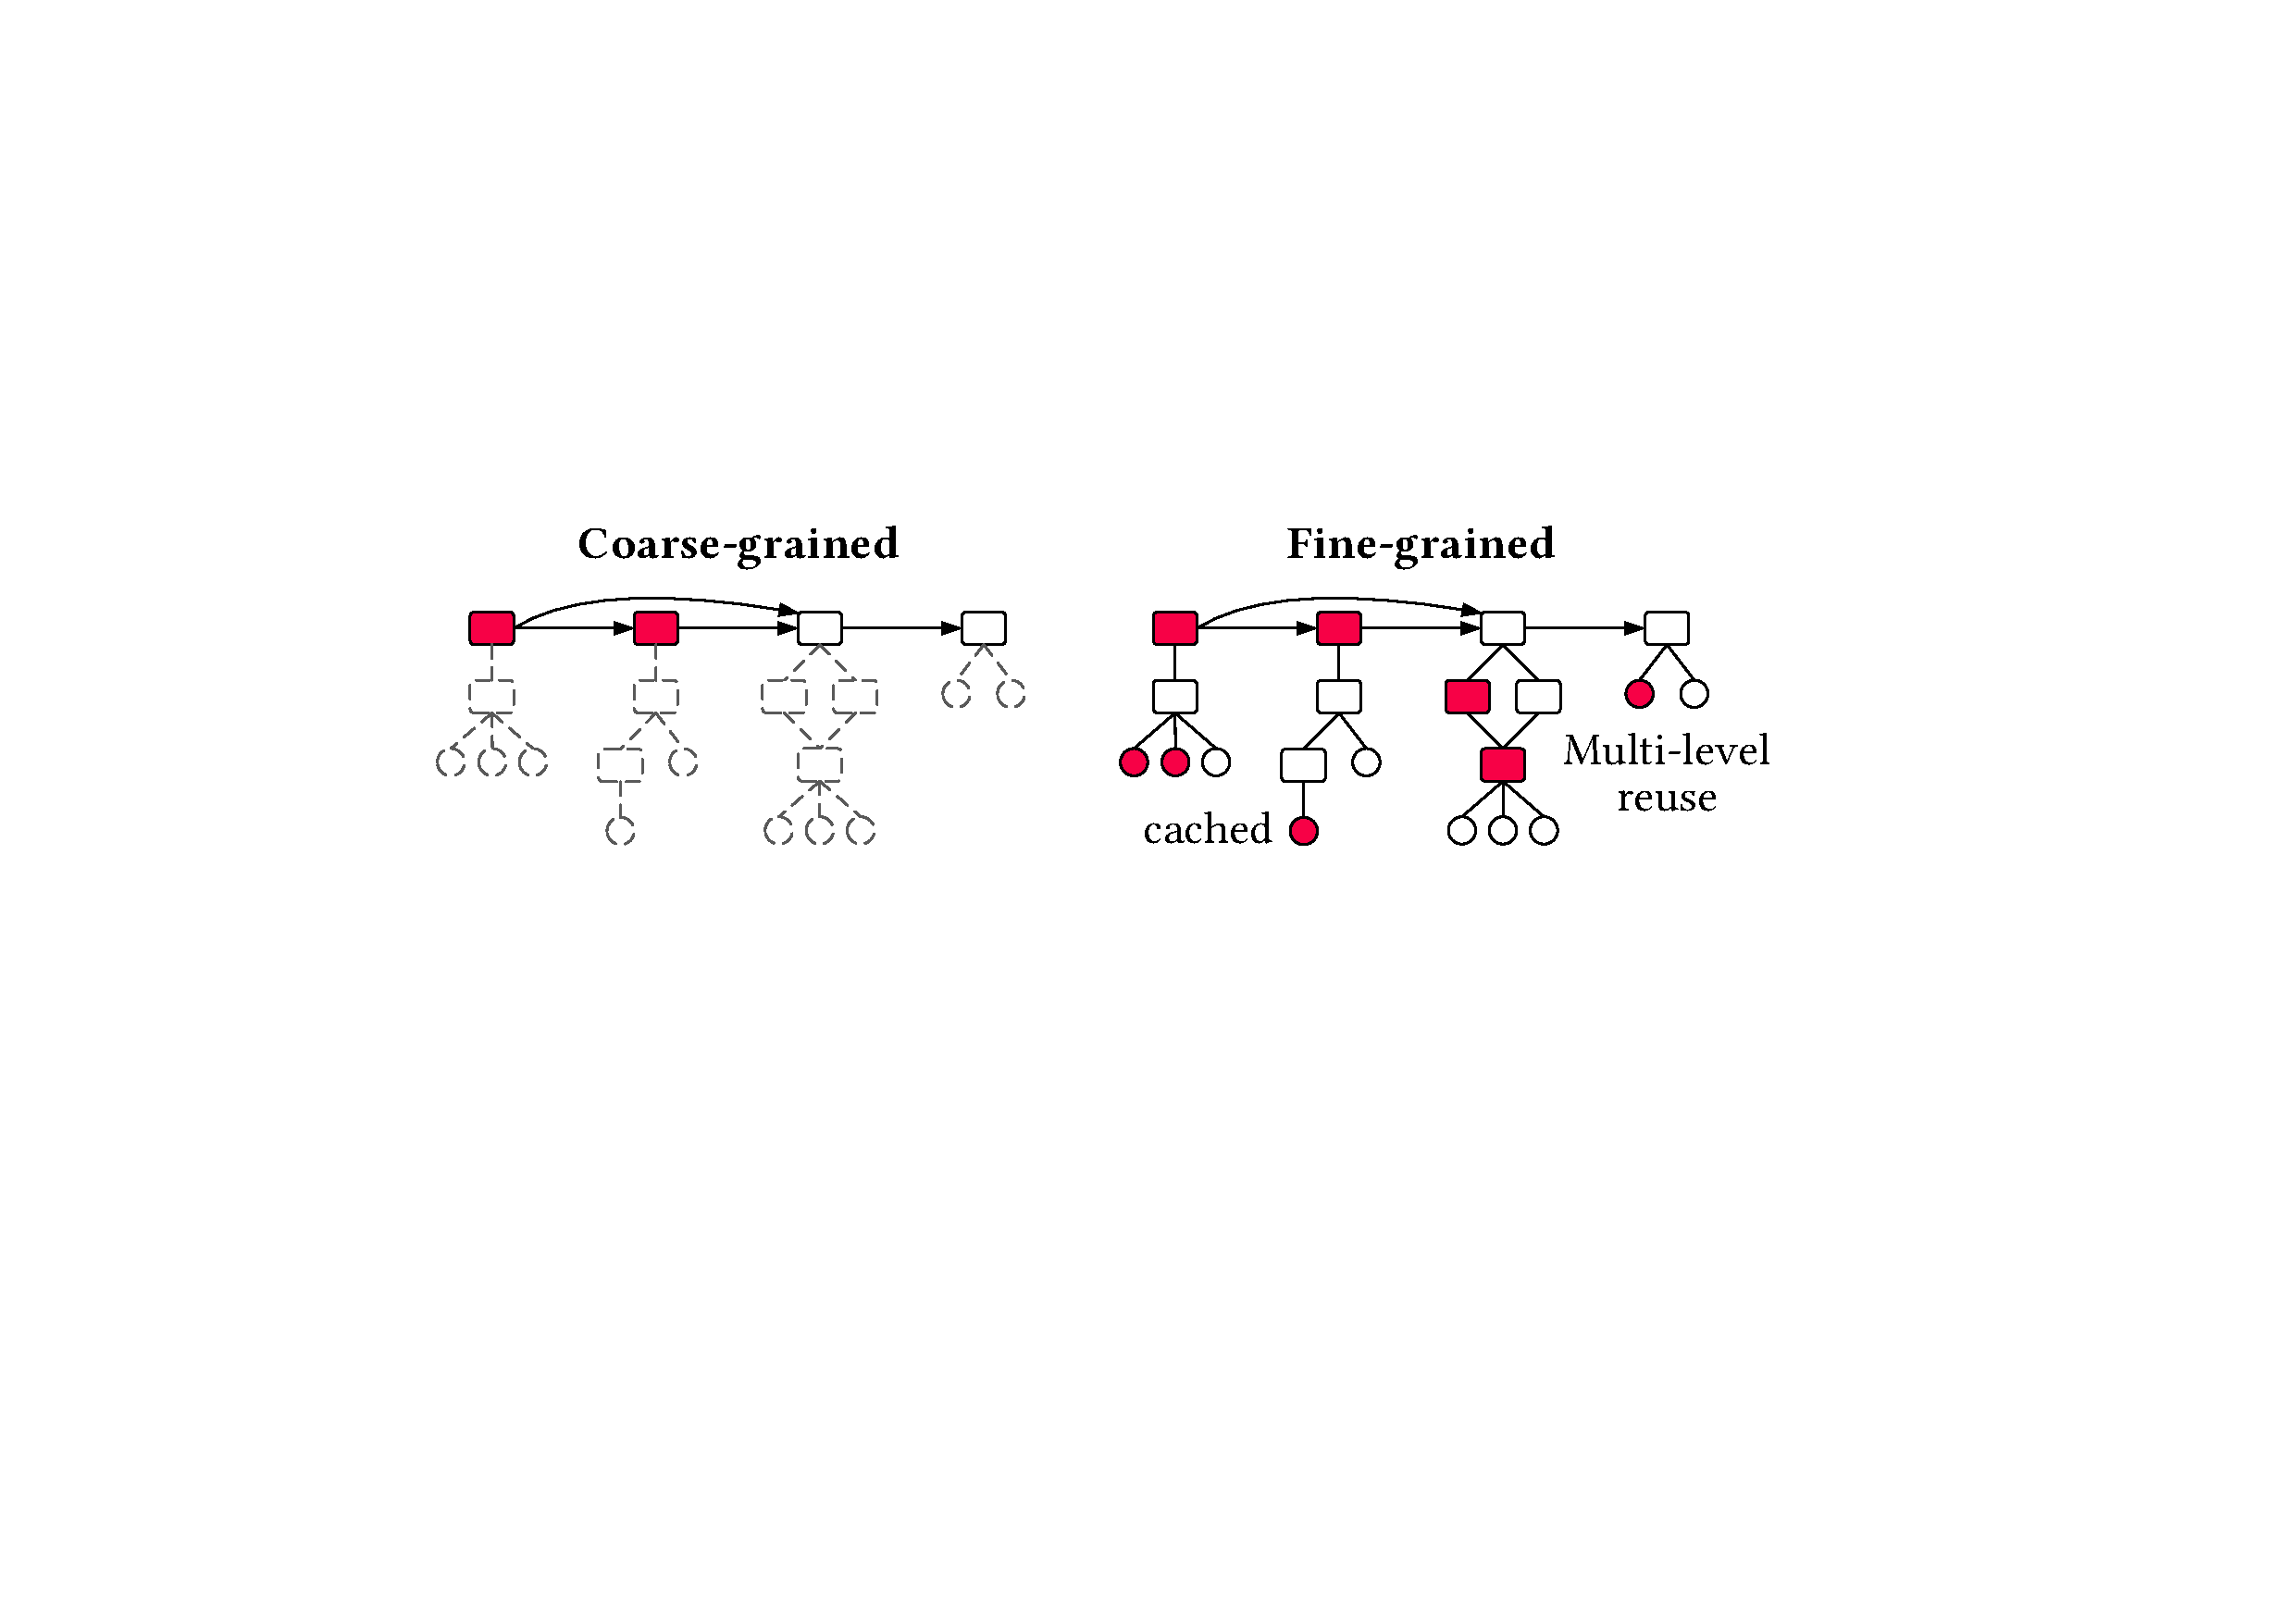
\includegraphics[scale=0.317]{figures/coarse_vs_fine2}
	\vspace{-0.25cm}
	\caption{\label{fig:coarsefine}Coarse- and Fine-grained Lineage-based Reuse {\normalfont(for ML pipelines, utilizing hierarchically composed building blocks)}.}
	\vspace{-0.1cm}
\end{figure}

% Problem 1: versioning, reproducibility, model management
\textbf{Problem of Non-Determinism:} Many ML primitives are non-deterministic, so multiple runs with the same inputs do not yield the same results. Examples are (1) ML algorithms with randomly initialized models, (2) random reshuffling of matrices for mini-batch algorithms, cross validation, data partitioning, and splitting, (3) drop-out layers for regularization in deep neural networks (DNNs), and (4) basic randomized operations like \texttt{rand} or \texttt{sample}. Interestingly, recent work has found significant impact of random seeds on the model accuracy of cutting-edge DNNs \cite{abs-2002-06305}. When computing lineage for high-level primitives, this internal non-determinism---unless exposed via seed parameters---quickly becomes invisible. Externally encoding this metadata is possible but again defeats the purpose of being independent of underlying ML systems and their implementation. Therefore, non-determinism limits the use of coarse-grained lineage for versioning, reproducibility, and reuse.

% Problem 2: lots of unnecessary redundancy
\textbf{Problem of Unnecessary Redundancy:} The repetitive nature of exploratory data science processes, and increasingly complex, hierarchically composed ML pipelines and workflows, create high computational redundancy. While coarse-grained reuse can eliminate redundancy of identical steps, it fails to eliminate fine-grained redundancy. First, existing ML libraries and systems often compose high-level primitives from smaller building blocks to ensure reuse and consistency. For example, Scikit-learn \cite{PedregosaVGMTGBPWDVPCBPD11} allows creating custom pipelines (via \texttt{make\_pipeline()}) from sequences of pre-processing steps and ML algorithms, and then feed these pipelines into high-level primitives like \texttt{GridSearchCV}. Since this composition is unaware of independent operations and substeps, (and hand-optimized primitives for all combinations are infeasible), we end up with unnecessary redundancy. Unfortunately, in general-purpose programming languages, this redundancy is very difficult to correctly detect and eliminate. Second, entire ML algorithms might be repeatedly used inside feature selection and cross validation primitives, which show an orthogonal type of partial redundancy due to incrementally added features (feature selection), removed features (debugging), or overlapping fold compositions.  

\textbf{LIMA Framework Overview:} Our LIMA framework overcomes these problems by a novel concept of \emph{fine-grained} lineage tracing and reuse \emph{inside} ML systems, as shown in Figure~\ref{fig:coarsefine}-right. We maintain a lineage DAG (directed acyclic graph) for all life variables during runtime of an ML program. Nodes represent executed operations---including parameters that make them deterministic (e.g., system-generated random seeds)---and edges are data dependencies. This DAG is recursively built, while executing conditional control flow and operations. The lineage of a variable exactly identifies an intermediate result, and can then be accessed, stored, and used to reproduce this intermediate. In order to eliminate unnecessary redundancy, we further leverage the lineage as keys in a reuse cache for full and partial reuse, with compensations for partial reuse. Figure~\ref{fig:coarsefine} shows the resulting reuse opportunities at the granularity of individual operations, control-flow blocks, and functions.

\textbf{Contributions:} Our main contribution is the LIMA framework for efficient, fine-grained lineage tracing and reuse, implemented in Apache SystemDS\footnote{The source code is available at \url{https://github.com/apache/systemds}.} \cite{BoehmADGIKLPR20} as a representative ML system. Key ideas of this approach, beyond state-of-the-art, are (1) multi-level lineage tracing and reuse, (2) full and partial reuse of intermediates, and (3) a robust integration with ML system internals such as task parallelism and operator fusion. Our technical contributions are:
\begin{itemize}
\item \emph{ML Systems Background:} To aid understanding, we provide the necessary background of ML system internals, and discuss different sources of redundancy in Section~\ref{sec:bg}.
\item \emph{Lineage Tracing:} We then define the concept of Lineage DAGs, and discuss multi-level lineage tracing in Section~\ref{sec:lic}. This discussion also includes the deduplication of lineage traces for functions, loops, blocks, and fused operators. 
\item \emph{Lineage-based Reuse:} Leveraging these lineage traces, we introduce techniques for full and partial reuse of intermediates in Section~\ref{sec:reuse}. This reuse infrastructure relies on compiler-assisted, cost-based runtime caching, tailor-made eviction policies, and thread-safe access in task-parallel programs.
\item \emph{Experiments:} Finally, we report on extensive experiments in Section~\ref{sec:exp} that show low overhead lineage tracing, and significant performance improvements, compared to baselines like TensorFlow~\cite{AbadiBCCDDDGIIK16} and HELIX~\cite{XinMMLSP18}, on various ML workloads.
\end{itemize}
 
